\documentclass[12pt, varwidth, border=5mm]{standalone}
\usepackage{tikz}
\usepackage{amsmath}
% Underlining package
\usepackage{ulem}
\usetikzlibrary{calc}
\usetikzlibrary{angles,quotes}
% \usepackage[a4paper, portrait, margin=1cm]{geometry}

\begin{document}
\section*{ }
    \begin{minipage}{0.55\textwidth}
  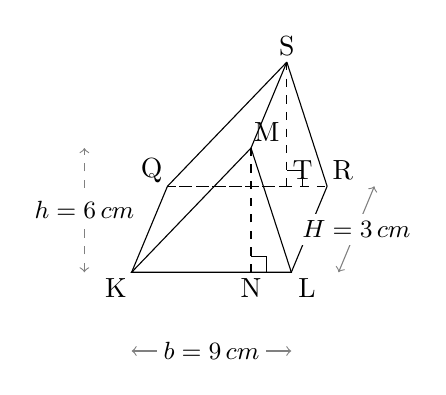
\begin{tikzpicture}[scale=1.0, baseline=(current bounding box.north)]
    \begin{scope}[rotate=0]

        \coordinate (K) at (0,0);
        \coordinate (L) at (2.028,0);
        \coordinate (N) at (1.516,0);
        \coordinate (M) at ($(N)+(0,1.577)$); % Perpendicular upwards


        % back face skew shift
        \coordinate (Q) at ($(K)+(0.455, 1.092)$);
        \coordinate (R) at ($(L)+(0.455, 1.092)$);
        \coordinate (S) at ($(M)+(0.455, 1.092)$);
        \coordinate (T) at ($(N)+(0.455, 1.092)$);


        \draw (K)--(L)--(M)--cycle;
        \draw[dashed] (N)--(M);
        \pic [draw, -, angle radius=0.2cm] {right angle=M--N--L};

        \draw[] (K)--(Q);
        \draw[] (L)--(R);
        \draw[] (M)--(S);

         \pic [draw, -, angle radius=0.2cm] {right angle=S--T--R};

        \draw[] (Q)--(S);
        \draw[dashed] (S)--(T);
        \draw[dashed] (Q)--(R);
        \draw[] (R)--(S);
        \draw[dashed] (T)--(Q);


        % Vertex LABELS
        % Labels relative to shape geometry
        \node at ($(K)+(-0.2,-0.2)$) {K};
        \node at ($(L)+(0.2,-0.2)$) {L};
        \node at ($(N)+(0.0,-0.2)$) {N};
        \node at ($(M)+(0.2,0.2)$) {M};

        \node at ($(Q)+(-0.2,0.2)$) {Q};
        \node at ($(R)+(0.2,0.2)$) {R};
        \node at ($(S)+(0.0,0.2)$) {S};
        \node at ($(T)+(0.2,0.2)$) {T};

        % dotted/dashed arrows shifted away from edges
        % Horizontal side (A-B), shifted down yshift=0mm,
        % {\small $b = 9\,cm$};
        \draw[<->, gray]
            ($(K) + (0,-1.0cm)$) -- ($(L) + (0,-1.0cm)$)
            node[black, midway, fill=white, inner sep=2.5pt] {\small $b = 9 \,cm$};

        % Vertical side (B-C), shifted right xshift=0mm,
        \draw[<->,dashed, gray]
            ($(K |- N)+(-0.6,0)$) -- ($(K |- M)+(-0.6,0)$)
            node[black, midway, fill=white, inner sep=2.5pt] {\small $h = 6 \,cm$};

        % depth (L-R),
        \draw[<->, gray]
            ($(L)+(0.6,0)$) -- ($(R)+(0.6,0)$)
            node[black, midway, fill=white, inner sep=2.5pt] {\small $H = 3 \,cm$};

    \end{scope}
\end{tikzpicture}
\end{minipage}%
\hfill
\begin{minipage}{.4\textwidth}
  \begin{align*}
    \text{Volume} &= \frac{1}{2} \text{bhH} \\
    \text{Volume} &= \frac{1}{2} \times 9 \,\text{cm} \times 6 \,\text{cm} \times 3 \,\text{cm} \\
    \text{Volume} &= 81.0 \text{cm}^3
  \end{align*}
\end{minipage}

\end{document}
